\documentclass{article}
\usepackage[utf8]{inputenc}
\usepackage{enumitem}
\usepackage{amsmath}
\usepackage{amsthm}
\usepackage{amssymb}
\usepackage{tikz}
\usepackage{standalone}
\newtheorem{theorem}{Theorem}[section]
\newtheorem{lemma}[theorem]{Lemma}
\setlength{\parskip}{1em}

%------------tikz Setup------------

\tikzstyle{ball} = [circle,shading=ball, ball color=black,
    minimum size=1mm,inner sep=1.3pt]
\tikzstyle{miniball} = [circle,shading=ball, ball color=black,
    minimum size=1mm,inner sep=0.5pt]
\tikzstyle{mminiball} = [circle,shading=ball, ball color=black,
    minimum size=0.6mm,inner sep=0.1pt]
\usetikzlibrary{arrows.meta}
\usetikzlibrary{angles, quotes}
\tikzset{>={Latex[length=2mm,width=1.5mm]}}
\tikzset{->-/.style={decoration={markings, mark=at position #1 with
  {\arrow{>}}},postaction={decorate}}}
\usetikzlibrary{decorations.pathmorphing}
\usetikzlibrary{decorations.pathreplacing}
\usetikzlibrary{arrows.meta,calc}
\usetikzlibrary{bending}
\usetikzlibrary{decorations.markings,shapes.geometric}
\tikzset{->-/.style={decoration={markings, mark=at position #1 with
  {\arrow{>}}},postaction={decorate}}}
\tikzset{-|-/.style={decoration={markings, mark=at position #1 with
  {\arrow{stealth}}},postaction={decorate}}}
\tikzset{movearrow/.style 2 args ={
        decoration={markings,
    mark= at position {#1} with {\arrow{#2}} ,
        },
        postaction={decorate}
    }
}

\renewcommand\qedsymbol{$\blacksquare$}

\title{REU 2021 - Problem Set 5}
\author{Kevin Y. Wu}
\date{\today}

\begin{document}

\maketitle

\pagenumbering{roman}
\tableofcontents
\newpage
\pagenumbering{arabic}


\section{Problem 1.}
For a permutation $\sigma\in \mathbb{S}_n$ we denote by $\textup{Inv}(\sigma)$ the number of inversions in $\sigma,$ namely the number of pairs $1\leq i<j\leq n$ such that $\sigma(i)>\sigma(j).$
\begin{enumerate}[label=(\alph*)]
    \item Find permutations in $\mathbb{S}_n$ with the smallest number of inversions and with the biggest number of inversions. 
    \par Smallest:
    $\begin{pmatrix}
    1 & 2 & \dots & n-1 & n\\
    1 & 2 & \dots & n-1 & n
    \end{pmatrix}$
    \par Biggest:
    $\begin{pmatrix}
    1 & 2 & \dots & n-1 & n\\
    n & n-1 & \dots & 2 & 1
    \end{pmatrix}$
    \item Prove that 
    \[\sum_{\pi \in \mathbb{S}_n} x^{\textup{Inv}(\pi)}=(1+x)(1+x+x^2)\dots (1+x+x^2+\dots+x^{n-1}).\]
    \begin{proof}
    We will prove the statement by induction.
    \par Base case. For $n=1$, 
    \[\sum_{\pi \in \mathbb{S}_1} x^{\textup{Inv}(\pi)}=x^0=1.\]
    For $n=2$, 
    \[\sum_{\pi \in \mathbb{S}_2} x^{\textup{Inv}(\pi)}=x^0+x^1=1+x.\]
    \par Inductive step. Suppose 
    \[\sum_{\pi \in \mathbb{S}_n} x^{\textup{Inv}(\pi)}=(1+x)(1+x+x^2)\dots (1+x+x^2+\dots+x^{n-1})\]
    is true. Then we must show
    \begin{align*}
        \sum_{\pi' \in \mathbb{S}_{n+1}} x^{\textup{Inv}(\pi')}
        &=(1+x)(1+x+x^2)\dots (1+x+x^2+\dots+x^{n})\\
        &=\left (\sum_{\pi \in \mathbb{S}_n} x^{\textup{Inv}(\pi)}\right )(1+x+x^2+\dots+x^{n})\\
        &=\sum_{\pi \in \mathbb{S}_n} x^{\textup{Inv}(\pi)}(1+x+x^2+\dots+x^{n}).
    \end{align*}
    \par Consider a permutation $\pi \in \mathbb{S}_n$. Then we can insert the $n+1$ element in the $i^{\textup{th}}$ position for $1\leq i\leq n+1$ and increase the indices of the elements to the right of $n+1$ by one. Call the new permutation $\pi'$. Since the $n+1$ element is now the largest in the set, inserting it in the $i^{\textup{th}}$ position adds $n+1-i$ inversions. Thus,
    \begin{align*}
        x^{\textup{Inv}(\pi')}
        &=x^{\textup{Inv}(\pi)}+x^{\textup{Inv}(\pi)+1}+x^{\textup{Inv}(\pi)+2}+\dots+x^{\textup{Inv}(\pi)+n}\\
        &=x^{\textup{Inv}(\pi)}(1+x+x^2+\dots+x^{n})
    \end{align*}
    Considering the summation of every $\pi \in \mathbb{S}_n$, we have 
    \[ \sum_{\pi' \in \mathbb{S}_{n+1}} x^{\textup{Inv}(\pi')}=\sum_{\pi \in \mathbb{S}_n} x^{\textup{Inv}(\pi)}(1+x+x^2+\dots+x^{n})\]
    as desired.
    \end{proof}
    \item Prove that numbers $\textup{Inv}(\sigma)$ and $\textup{Inv}(\sigma^{-1})$ have the same parity.
    \begin{proof}
    By problem 3(b) of Problem Set 1, every permutation is a product of transposition. Then we can write 
    \begin{align*}
        \sigma &= \tau_1\tau_2\dots\tau_n\\
        \sigma^{-1} &= \tau_n^{-1}\tau_{n-1}^{-1}\dots\tau_1^{-1}.
    \end{align*}
    A single transposition either increases or decreases the number of inversions by one, thus changing the parity. If the two elements are not already inverted, applying the transposition inverts them, and vice versa. It follows that applying two transpositions on a permutation does not change the parity of inversions. To get from $\sigma$ to $\sigma^{-1}$, we can see that 
    \begin{align*}
        \sigma(\sigma^{-1})^2 &= (\tau_1\tau_2\dots\tau_n)(\tau_n^{-1}\tau_{n-1}^{-1}\dots\tau_1^{-1})^2\\
        &=e(\tau_n^{-1}\tau_{n-1}^{-1}\dots\tau_1^{-1})\\&=\sigma^{-1}.
    \end{align*}
    Thus, we must apply $2n$ transpositions. We can apply two transpositions at a time for $n$ times, so $\textup{Inv}(\sigma)\equiv \textup{Inv}(\sigma^{-1})\pmod{2}$.
    \end{proof}
\end{enumerate}


\section{Problem 2.}
A bijection $f \colon \mathbb{R}^2\rightarrow \mathbb{R}^2$ such that there exists $k>0$ such that
\[|f(A)f(B)|=k|AB|\]
is called a {\it similarity}.
\begin{enumerate}[label=(\alph*)]
    \item Prove that homothety $H_O^{\lambda}$ is a similarity. \label{2c}
    \begin{proof}
    Let $H_O^{\lambda}(A)=A'$ and $H_O^{\lambda}(B)=B'$. We need to prove that $|A'B'|=\lambda|AB|$ for any segment $\overline{AB}$. Consider the following cases.
    \begin{enumerate}[label=(\alph*)]
        \item Point $O$ lies on the same line as $A$ and $B$, between $A$ and $B$. Then $|OA'|=\lambda|OA|$ and $|OB'|=\lambda|OB|$. Then we have $|A'B'|=|OA'|+|OB'|=\lambda|OA|+\lambda|OB|=\lambda|AB|$, as desired.
        
        \begin{figure}[h]
            \centering
            \input{images/2c_1}
            \caption{$\lambda=2$}
        \end{figure}
        
        \item Point $O$ lies on the same line as $A$ and $B$, one one side of $A$ and $B$. Then $|OA'|=\lambda|OA|$ and $|OB'|=\lambda|OB|$. Suppose, without loss of generality, that $O$ is closest to $B$. Then we have $|A'B'|=|OA'|-|OB'|=\lambda|OA|-\lambda|OB|=\lambda|AB|$, as desired.
        
        \begin{figure}[h]
            \centering
            \documentclass{standalone}
\usepackage{tikz}
%------------tikz Setup------------

\tikzstyle{ball} = [circle,shading=ball, ball color=black,
    minimum size=1mm,inner sep=1.3pt]
\tikzstyle{miniball} = [circle,shading=ball, ball color=black,
    minimum size=1mm,inner sep=0.5pt]
\tikzstyle{mminiball} = [circle,shading=ball, ball color=black,
    minimum size=0.6mm,inner sep=0.1pt]
\usetikzlibrary{arrows.meta}
\usetikzlibrary{angles, quotes}
\tikzset{>={Latex[length=2mm,width=1.5mm]}}
\tikzset{->-/.style={decoration={markings, mark=at position #1 with
  {\arrow{>}}},postaction={decorate}}}
\usetikzlibrary{decorations.pathmorphing}
\usetikzlibrary{decorations.pathreplacing}
\usetikzlibrary{arrows.meta,calc}
\usetikzlibrary{bending}
\usetikzlibrary{decorations.markings,shapes.geometric}
\tikzset{->-/.style={decoration={markings, mark=at position #1 with
  {\arrow{>}}},postaction={decorate}}}
\tikzset{-|-/.style={decoration={markings, mark=at position #1 with
  {\arrow{stealth}}},postaction={decorate}}}
\tikzset{movearrow/.style 2 args ={
        decoration={markings,
    mark= at position {#1} with {\arrow{#2}} ,
        },
        postaction={decorate}
    }
}


\begin{document}
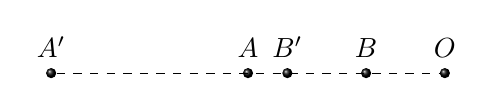
\begin{tikzpicture}
\begin{scope}[scale=1]
    %points
    \node[ball, label={$O$}] (o) at (0,0) {};
    \node[ball, label={$A$}] (a) at (-2.5,0) {};
    \node[ball, label={$B$}] (b) at (-1,0) {};
    \node[ball, label={$A'$}] (a') at (-5,0) {};
    \node[ball, label={$B'$}] (b') at (-2,0) {};
    \draw[dashed] (a') to (o);
\end{scope}
\end{tikzpicture}
\end{document}
            \caption{$\lambda=2$}
        \end{figure}
        
        \item Point $O$ does not lie on the same line as $A$ and $B$. Then $AOB$ and $A'OB'$ are triangles. Let $\lambda<1$ (the case where $
        \lambda>1$ is similar). Then $A'$ lies on $\overline{OA}$ and $B'$ lies on $\overline{OB}$, so we have $\frac{\overline{OA'}}{\overline{OA}}=\frac{\overline{OB'}}{\overline{OB}}=\lambda$. By Thale's theorem, this implies that $\overline{AB}\parallel \overline{A'B'}$; furthermore, $\frac{|A'B'|}{|AB|}=\lambda$, as desired.
        
        \begin{figure}[h]
            \centering
            \input{images/2c_3}
            \caption{$\lambda=0.5$}
        \end{figure}
        
        Thus, homothety $H_O^{\lambda}$ is equivalent to a similarity of ratio $\lambda$.
    \end{enumerate}
    \end{proof}
    \item Prove that every similarity is a composition of a homothety and an isometry.
    \begin{proof}
    First, consider a composition $T_{\lambda}\circ H_O^{\lambda^{-1}}$, where $T_{\lambda}$ is a similarity with ratio $\lambda$ and $H_O^{\lambda^{-1}}$ is a homothety. From \ref{2c}, we have shown that homothety $H_O^{\lambda^{-1}}$ is equivalent to a similarity with ratio $\lambda^{-1}$. Thus, this composition is a similarity transformation with ratio $\lambda^{-1}\lambda=1$, which is an isometry, $I$. Furthermore, $H_O^{\lambda^{-1}}$ is invertible, and its inverse is $H_O^{\lambda}$.
    \begin{align*}
        I=T_{\lambda}\circ H_O^{\lambda^{-1}}.\\
        I\circ H_O^{\lambda}=T_{\lambda}\circ H_O^{\lambda^{-1}}\circ H_O^{\lambda}.\\
        I\circ H_O^{\lambda}=T_{\lambda}.
    \end{align*}
    Next, consider a composition $H_O^{\lambda^{-1}}\circ T_{\lambda}$, the commutative expression of $T_{\lambda}\circ H_O^{\lambda^{-1}}$. This composition is a similarity transformation with ratio $\lambda\lambda^{-1}=1$, which is an isometry, $I'$. Furthermore, $H_O^{\lambda^{-1}}$ is invertible, and its inverse is $H_O^{\lambda}$.
    \begin{align*}
        I'=H_O^{\lambda^{-1}}\circ T_{\lambda}.\\
        H_O^{\lambda}\circ I' =H_O^{\lambda}\circ H_O^{\lambda^{-1}}\circ T_{\lambda}.\\
        H_O^{\lambda}\circ I'=T_{\lambda}.
    \end{align*}
    \end{proof}
\end{enumerate}


\section{Problem 3.}
Prove that a composition of two homotheties with coefficients $\lambda_1, \lambda_2$ and center $O$ with $\lambda_1 \lambda_2 \neq 1$ is a homothety with coefficient $\lambda_1 \lambda_2.$
\begin{proof}
We have the following two homotheties
\begin{align*}
    H_O^{\lambda_1}(X)=X'&:\frac{\overline{OX'}}{\overline{OX}}=\lambda_1\\
    H_O^{\lambda_2}(X')=X''&:\frac{\overline{OX''}}{\overline{OX'}}=\lambda_2.
\end{align*}
Then
\[(H_O^{\lambda_2}\circ H_O^{\lambda_1})(X)=X'':\frac{\overline{OX''}}{\overline{OX}}=\frac{\overline{OX''}}{\overline{OX'}}\times \frac{\overline{OX'}}{\overline{OX}}=\lambda_2\lambda_1.\]
Hence, we have
\[H_O^{\lambda_2}\circ H_O^{\lambda_1}=H_O^{\lambda_2\lambda_1}.\]
\end{proof}


\section{Problem 4.}
Let $R_n$ denote a set of fixed point free permutations($\sigma(i)\neq i$ for $1\leq i \leq n$) in $\mathbb{S}_n.$ Prove that
\[\lim_{n \rightarrow \infty}\frac{|R_n|}{n!} =\frac{1}{e}.\]
\begin{proof}
By the Inclusion-Exclusion principle in problem 4 of Problem Set 2, we can count $|R_n|$. For $1\leq k\leq n$, denote $S_k$ as the set of permutations that have a fixed point at $k$. Then
\begin{align*}
    |R_n|
    &=|\mathbb{S}_n|-\sum_i |S_i| + \sum_{i<j} |S_i\cap S_j| +...+(-1)^n|S_1\cap \dots \cap S_n|\\
    &=\binom{n}{0}n!-\binom{n}{1}(n-1)!+\binom{n}{2}(n-2)!+\dots+(-1)^n\binom{n}{n}(n-n)!\\
    &=\sum_{i=0}^n(-1)^i\binom{n}{i}(n-i)!\\
    &=\sum_{i=0}^n(-1)^i\frac{n!}{i!(n-i)!}(n-i)!\\
    &=n!\sum_{i=0}^n\frac{(-1)^i}{i!}.
\end{align*}
Pluggin this into the limit, we have
\begin{align*}
    \lim_{n \rightarrow \infty}\frac{|R_n|}{n!}
    &=\lim_{n \rightarrow \infty}\frac{n!\sum_{i=0}^n\frac{(-1)^i}{i!}}{n!}\\
    &=\lim_{n \rightarrow \infty}\sum_{i=0}^n\frac{(-1)^i}{i!}\\
    &=\sum_{i=0}^{\infty}\frac{(-1)^i}{i!}.
\end{align*}
The power series for $e^x$ is $\sum_{i=0}^{\infty}\frac{x^i}{i!}$, so letting $x=-1$ gives us
\[\frac{1}{e}=e^{-1}=\sum_{i=0}^{\infty}\frac{(-1)^i}{i!}=\lim_{n \rightarrow \infty}\frac{|R_n|}{n!}.\]
\end{proof}


\end{document}
